
%--------------- Personalize your document here ---------------

\author{Emmanuel Rockwell} % Enter your name
\newcommand{\supervisorone}{Vincent Toups} % Enter your supervisor's name
\newcommand{\supervisortwo}{}% Leave it empty or enter your second supervisor's name 
\newcommand{\department}{UNIVERISTY OF NORTH CAROLINA -- CHAPEL HILL\\ Department of Biostatistics}
\newcommand{\exam}{BIOS 611 FINAL PROJECT}

\title{Pitchfork Analysis} %Enter the title of your report 
\date{November 2021} % insert a specific date	



\documentclass[a4paper,12pt]{article}
\usepackage[left=30mm,top=30mm,right=30mm,bottom=30mm]{geometry}
\usepackage{etoolbox} %required for cover page
\usepackage{booktabs}
\usepackage[usestackEOL]{stackengine}
\usepackage[T1]{fontenc}
\usepackage[utf8]{inputenc}
\usepackage{bm}
\usepackage{graphicx}
\usepackage{subcaption}
\usepackage{amsmath}
\usepackage{amsfonts}
\usepackage{mathtools}
\usepackage{xcolor}
\usepackage{float}
\usepackage{hyperref}
\usepackage[capitalise]{cleveref}
\usepackage{enumitem,kantlipsum}
\usepackage{amssymb}
\usepackage[square,numbers,sort]{natbib}
\usepackage[ruled,vlined]{algorithm2e}
\usepackage{listings}
%\usepackage{minted}
%\usemintedstyle{emacs}

%\renewcommand{\listingscaption}{Algorithm}
%\renewcommand{\listoflistingscaption}{List of Algorithms}


%\bibliographystyle{unsrtnat}

\hypersetup{
	colorlinks,
	linkcolor={black},
	citecolor={blue!50!black},
	urlcolor={blue!80!black}
}

\linespread{1}

\newtheorem{theorem}{Theorem}[section]
\graphicspath{{figures/}}	

%----------------------------------TITLE PAGE -----------------------------------
\makeatletter
\def\maketitle{
	\begin{center}\leavevmode
		\normalfont
		%\includegraphics[width=0.35\columnwidth]{queenslogo.pdf}
		\vskip 0.5cm   
		\textsc{\large \department}\\
		\vskip 1cm
		\includegraphics[width = 0.4\linewidth]{"unc_seal.png"}
		\vskip 1cm
		\rule{\linewidth}{0.2 mm} \\
		{\large \exam}\\[1 cm]
		{\huge \bfseries \@title \par}
		\vspace{1cm}
		\rule{\linewidth}{0.2 mm} \\[1.5 cm]
		
		\begin{minipage}[t]{0.45\textwidth}
			\begin{flushleft} \large
				\emph{Author:}\\
				\@author
			\end{flushleft}
		\end{minipage}
		\begin{minipage}[t]{0.45\textwidth}
			\begin{flushright} \large
				\ifdefempty{\supervisortwo}{\emph{Instructor:\\}}{\emph{Instructor:\\}}
				\supervisorone\\
				\ifdefempty{\supervisortwo}{}{\supervisortwo\\}
			\end{flushright}
		\end{minipage}
		\vfill
		{\Large \@date\par}
	\end{center}
	%\vfill
	%\null
	\cleardoublepage
}
\makeatother


%-------------------------------- ENDTITLE PAGE ----------------------------------

\begin{document}
	
	\pagenumbering{gobble}% Remove page numbers (and reset to 1)
	
	\maketitle
	
	\tableofcontents

	\newpage
	%\listoffigures
	%\newpage
	%\listoftables
	%\newpage
	%\listofalgorithms % List of algorithms in pseudocode format
	%\newpage
	%\listoflistings % List of algorithms in code format
	%\newpage
	
	
	\pagenumbering{arabic}% Arabic page numbers (and reset to 1)
	
	% This is how you can organize your document
\section{Introduction}
Founded in 1995, Pitchfork is an online music \& culture website that also organized the annual Pitchfork Music Festival in Chicago, IL. However, Pitchfork is mainly known for it's album reviews. Rather than assigning some amount of stars, thumbs-up, or tomatoes, Pitchfork aims to pursue a further degree of objective precision to its reviews -- assigning to each album a score on a 101-point scale between 0.0 and 10.0. 

Pitchfork's brand has evolved over the years. For the first 20 years or so of its existence, Pitchfork was mostly a mainstay of more alternative and underground music scenes, developing a reputation a reputation for it's somewhat contrarian opinions regarding popular music. However, in 2015 Pitchfork was sold to the media conglomerate Conde Nast and with the acquisition morphed into a mouthpiece for the music industries top record labels. 

To analyze Pitchfork's reviews, I used a dataset from components.one that scraped every pitchfork review between 1999 and January, 2019. 



\section{Score Distributions}
Perhaps the most interesting aspect of Pitchfork's reviews is the 101-point scale along which each album is evaluated. While this scale attempts to achieve a semblance of objectivity in reviews, very little is known about the methodology used when scores are assigned. Can we expect the average score to be a 5.0? What distribution of scores should we expect? How rare are very high and very low scores? Pitchfork doesn't disclose any of this information, so we're left to analyze the data ourselves to understand what the distribution of scores look like. Figure 1 shows the general distribution of the scores.

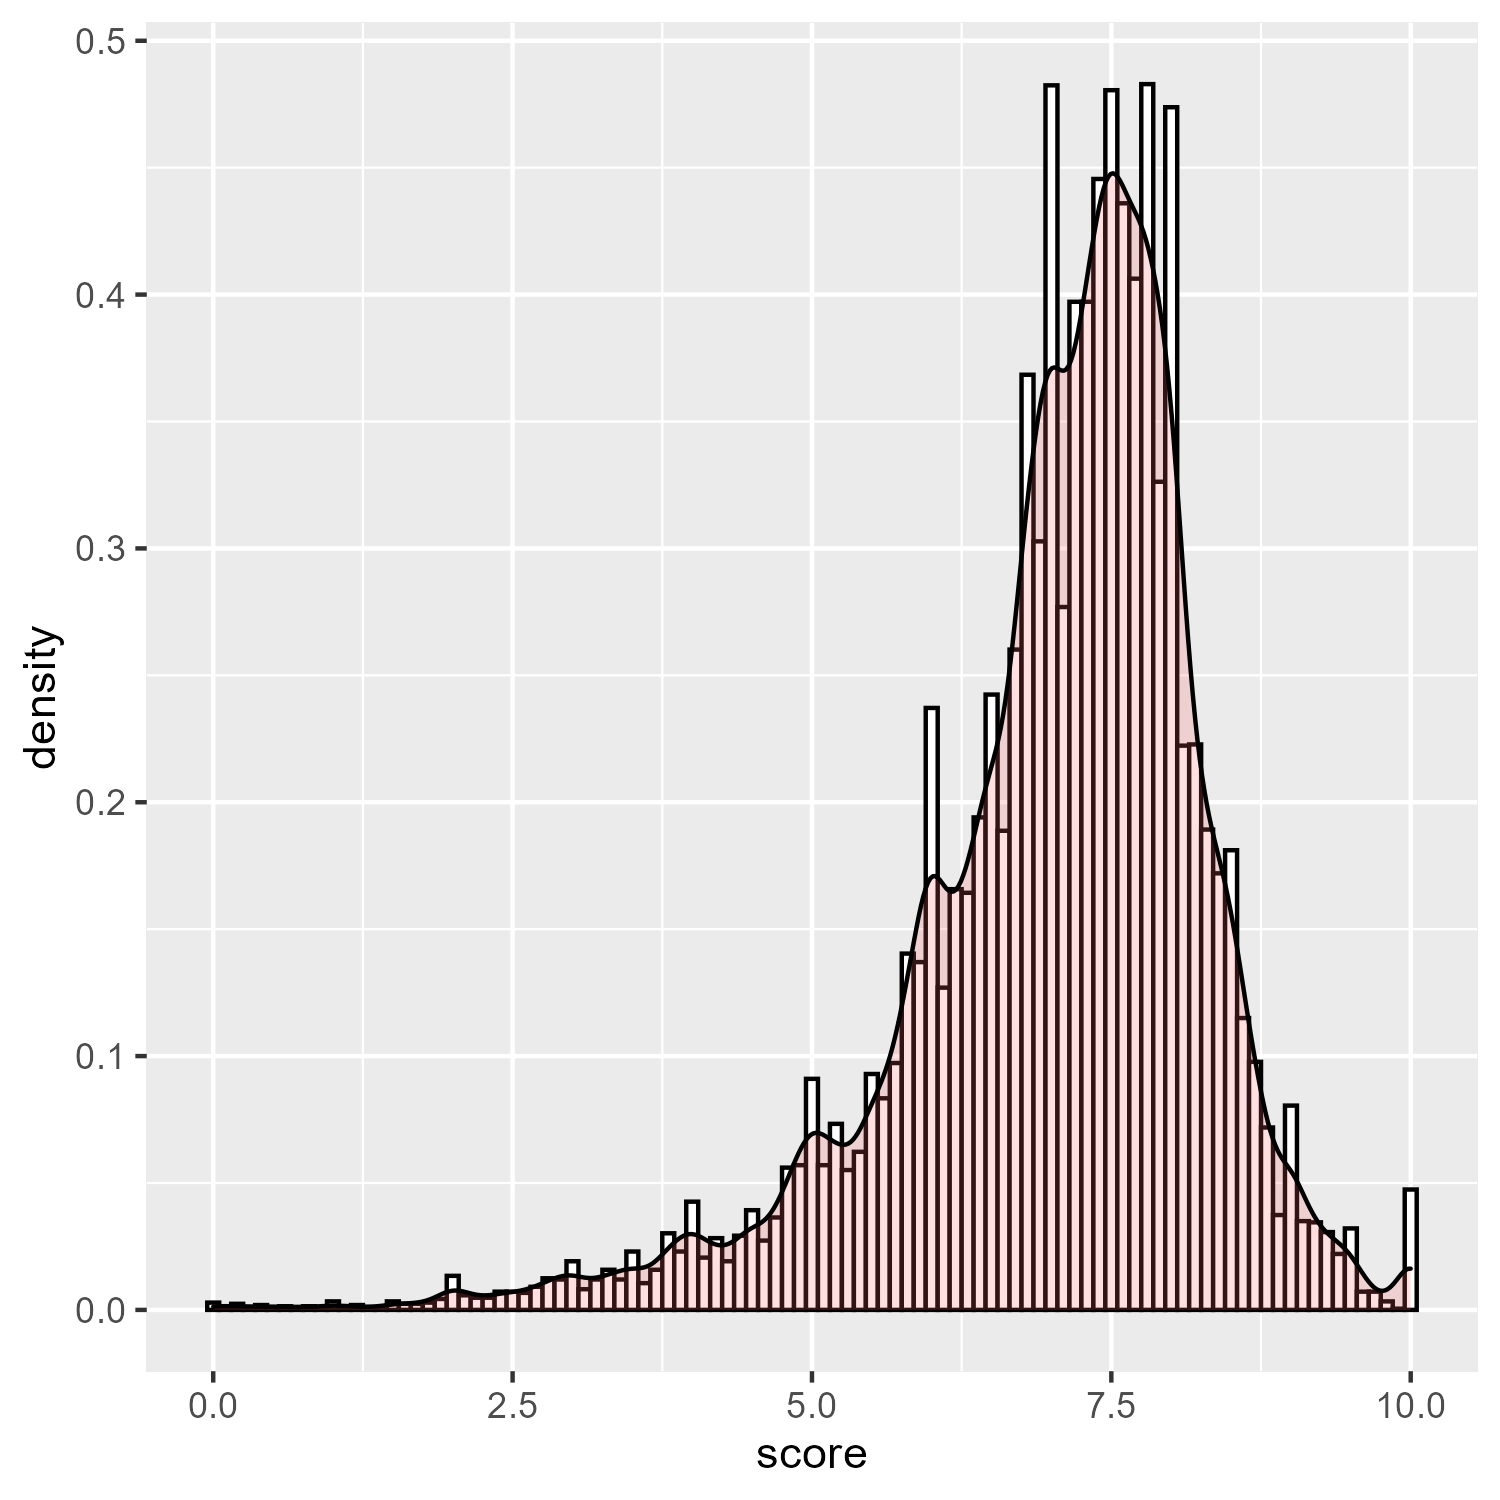
\includegraphics[width = \linewidth]{"figures/score_distribution.png"}

As we can see, scores seem to follow a left-skewed normal distribution. The mean score is 7.04 and the median score is 7.3. Therefore, a score is below-average and therefore "bad" relative to other albums if it has a score less than 7. A significant difference from the implicit assumption that 5 is the mean score. If this were the aim of the publication, they should attempt to be less favorable in their reviews. 
\subsection{Evaluating Score Objectivity}
Next I'd like to look at some interesting trends within the histogram -- specifically certain scores that are underindexed and overindexed empirically compared to what we would assume the theoretical distribution. 

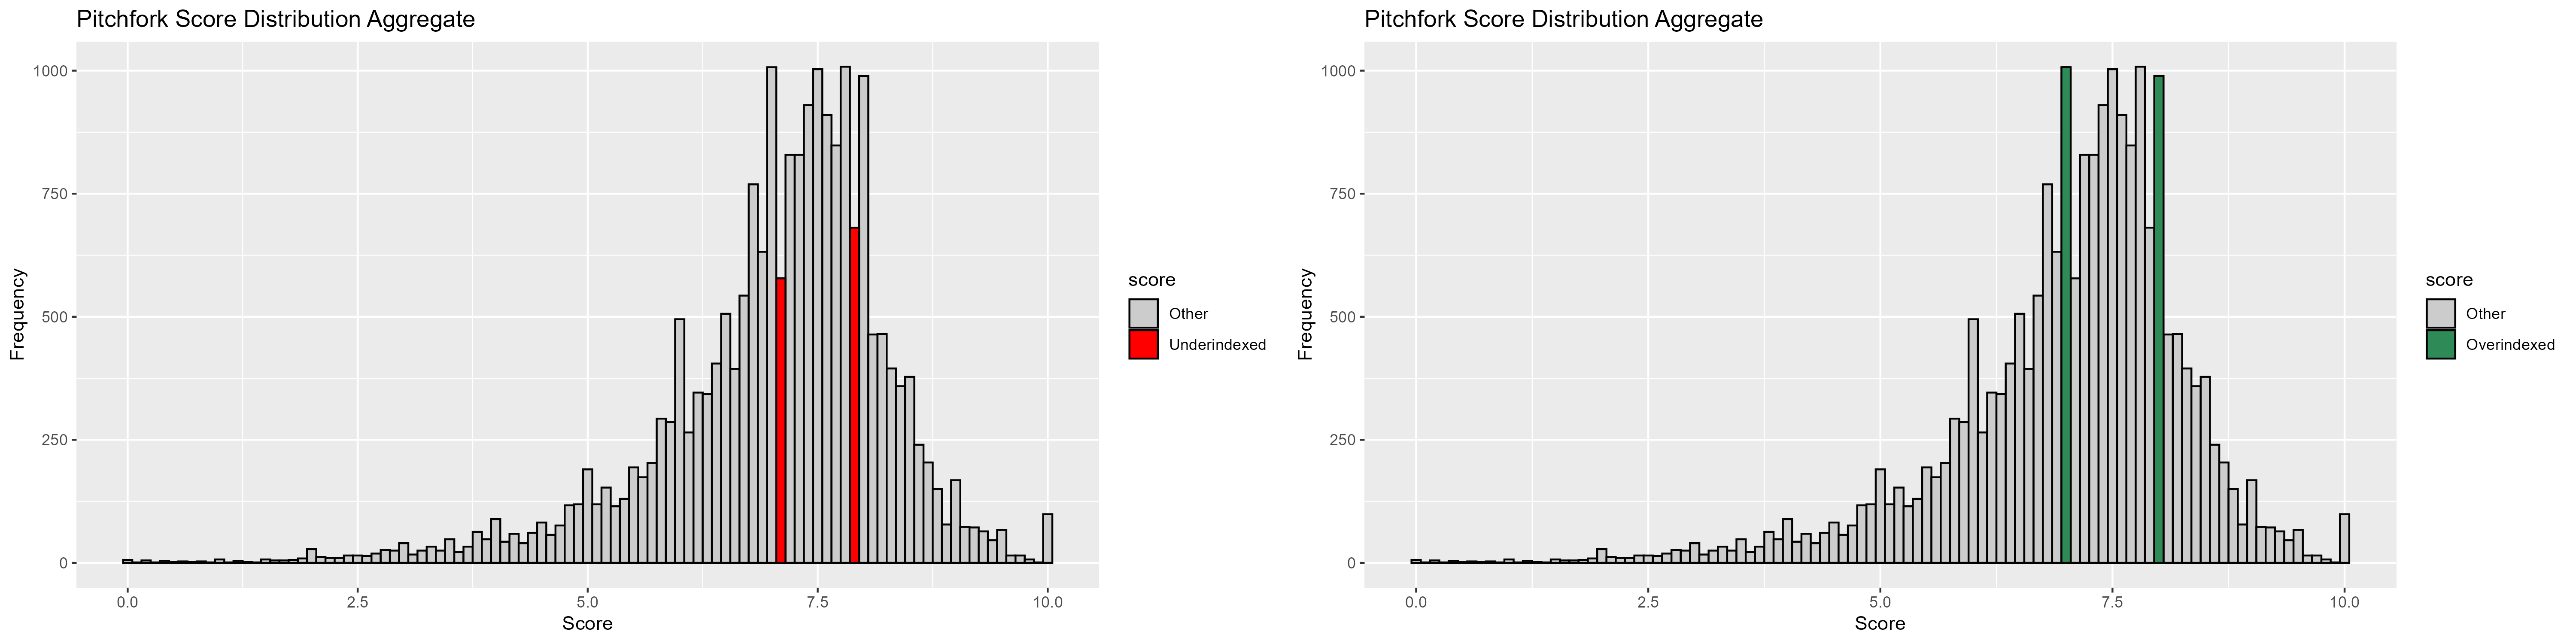
\includegraphics[width = \linewidth]{"figures/underoverindexing.png"}

The above figure highlights certain scores more or less prevalent in the empirical distribution than one would expect to find. Curiously, round numbers seem to be the most overindexed, with 7.0 and 8.0 both nearly matching the mode. On the other hand, scores like 7.1 and 7.9, while closer to the mode than 7.0 and 8.0, are significantly underrepresented in the data. Perhaps this reveals the more "human" aspect of this scoring convention. Since 7.1 and 7.9 seem like numbers that "lead" to 7.0 and 8.0 respectively, it appears that writers will unconsciously round down or round up when evaluating albums. 

\subsection{Distribution by Genre}

Finally, let's take a look at score distributions by genre. Pitchfork assigns multiple genres to albums -- often with many of the secondary genres being obscure. I simplified the issue by only taking the first genre listed on the website. This assumes that the first genre listed is the "primary" genre, which I believe is a fair assumption. 

I first wanted to understand whether Pitchfork writes more favorable reviews for certain genres. One can measure this by calculating the average score by genres and seeing how much this differs from the average score of 7.04. Furthermore, do the distribution of scores for specific genres differ significantly from the overall distribution? The below figures attempt to answer these questions: 

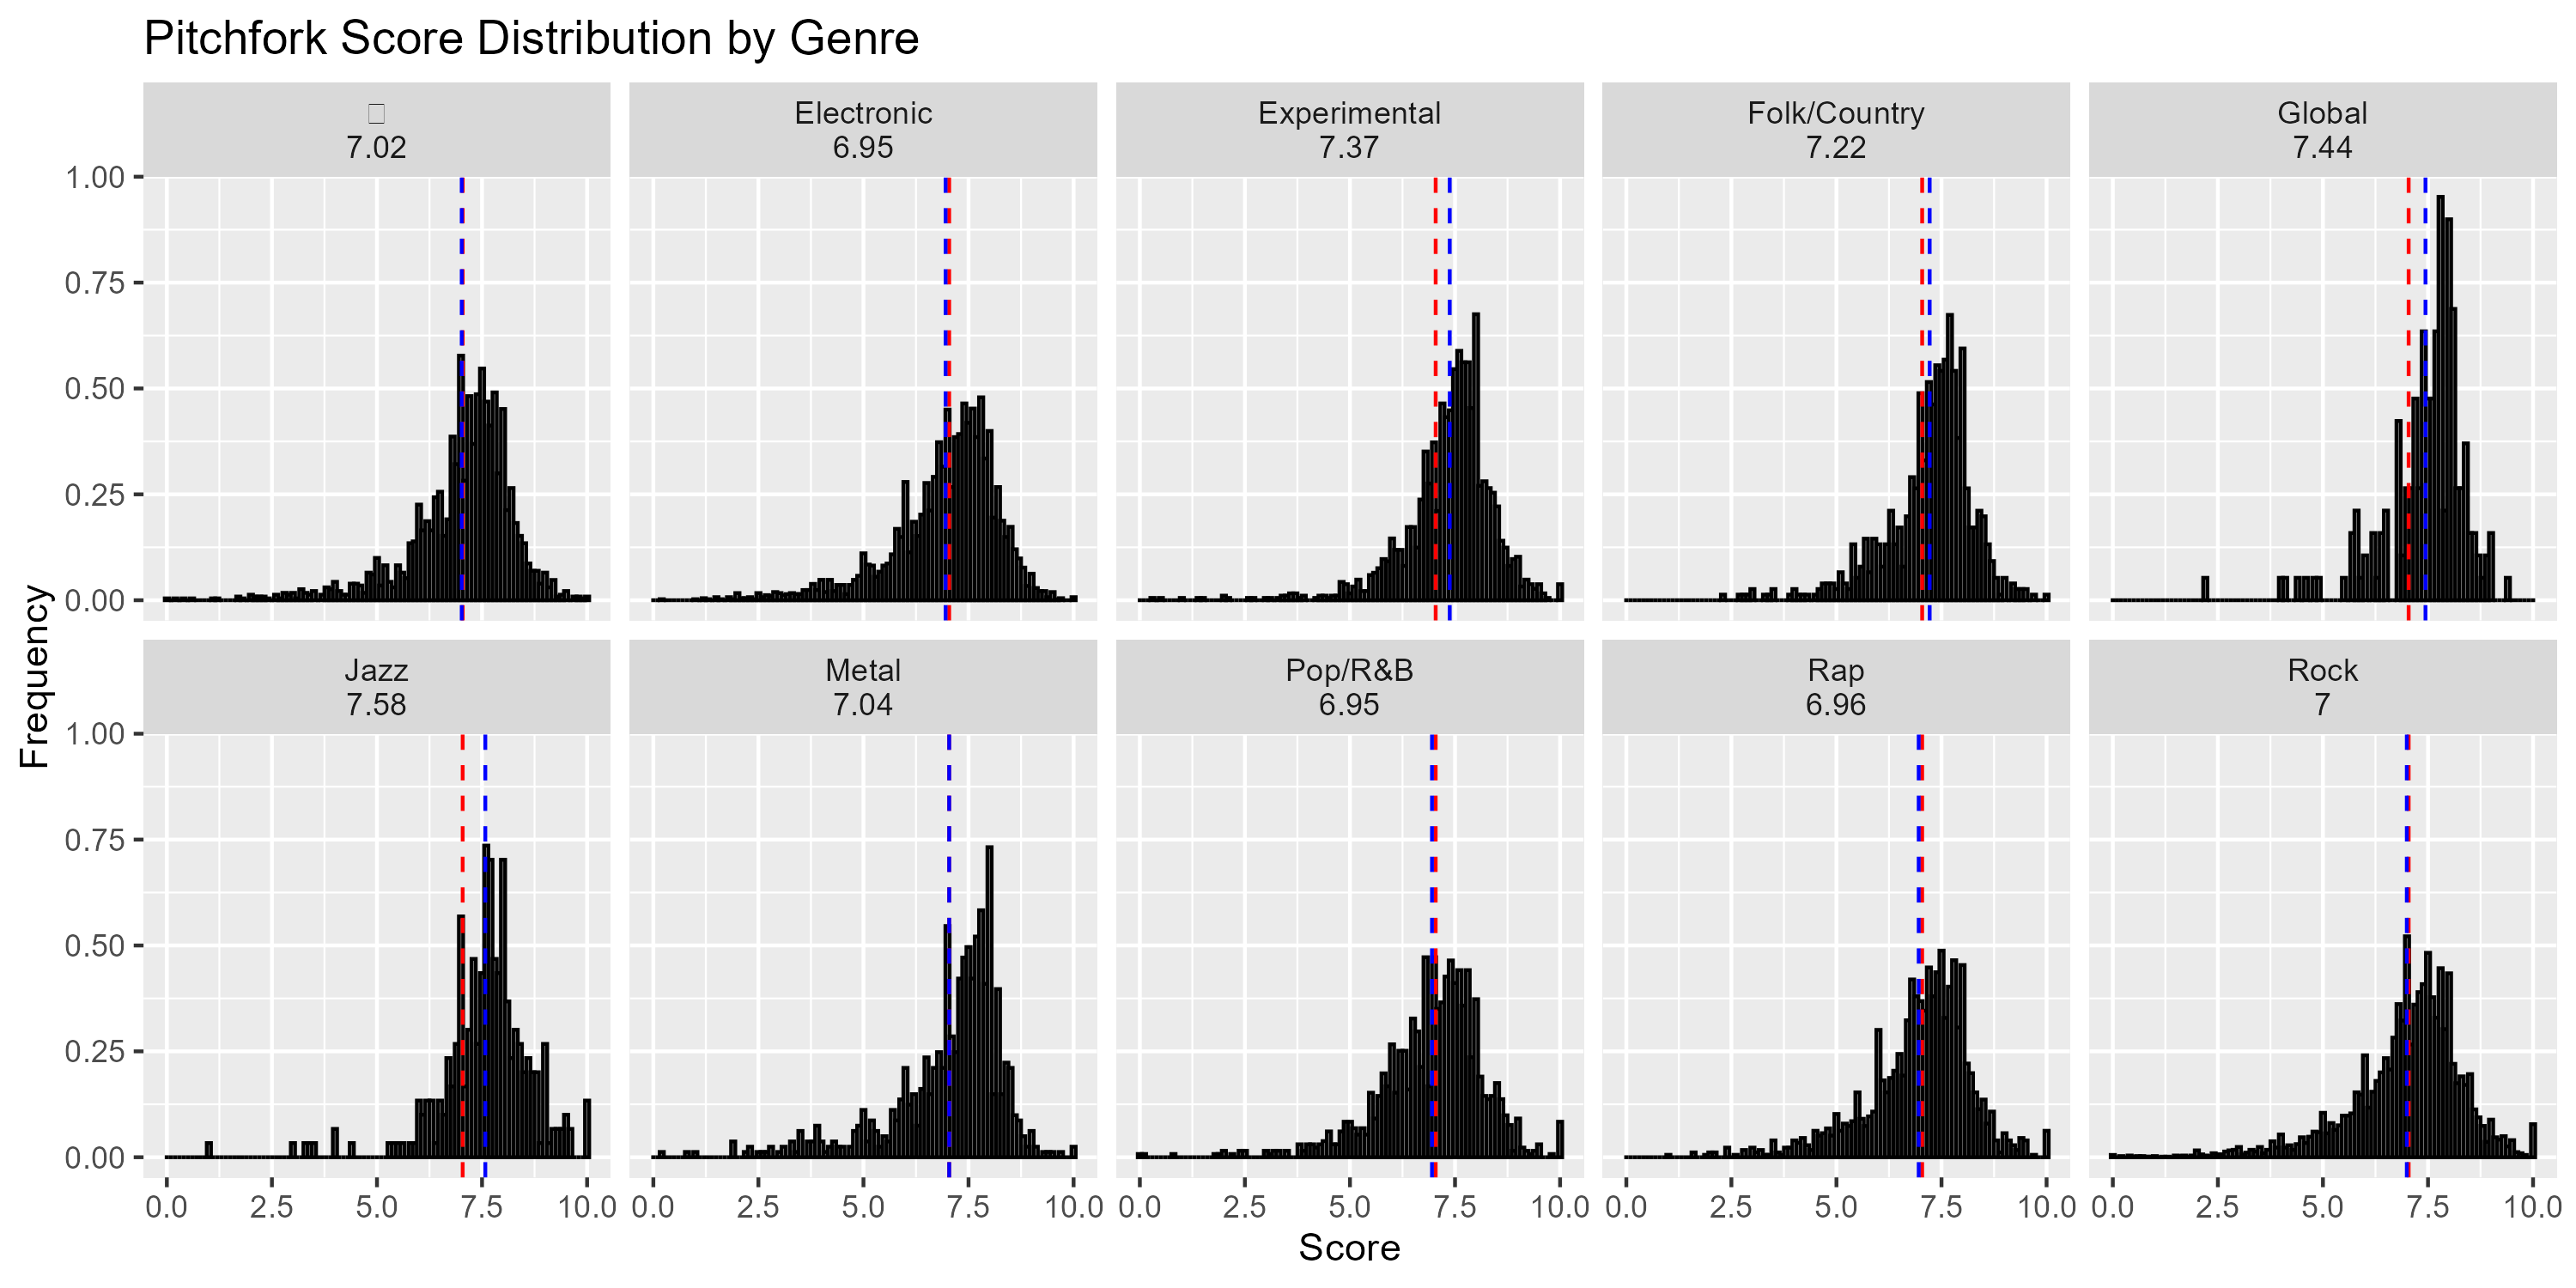
\includegraphics[width = \linewidth]{"figures/score_dist_by_genre.png"}

Note that the first histogram represents all albums without a listed genre. Albums with no genre represented about 10\% of albums and the average rating on these albums was consistent with the overall average. Pitchfork apparently provides higher scores on average to Jazz, Global, Experimental, and Folk/Country albums. On the other hand, Pitchfork gives it's least favorable reviews (on average) to Pop/R\&B, Electronic, and Rap albums. However, the low scores on these albums appear to be due to a longer tail than the Jazz, Global, Experimental, and Folk/Country album distributions. Therefore, I would conclude that Pitchfork likely doesn't rate these albums lower on average, but rather has a lower threshold for what constitutes 

\section{The Contrarian Index - Pitchfork Scores of Popular Music}
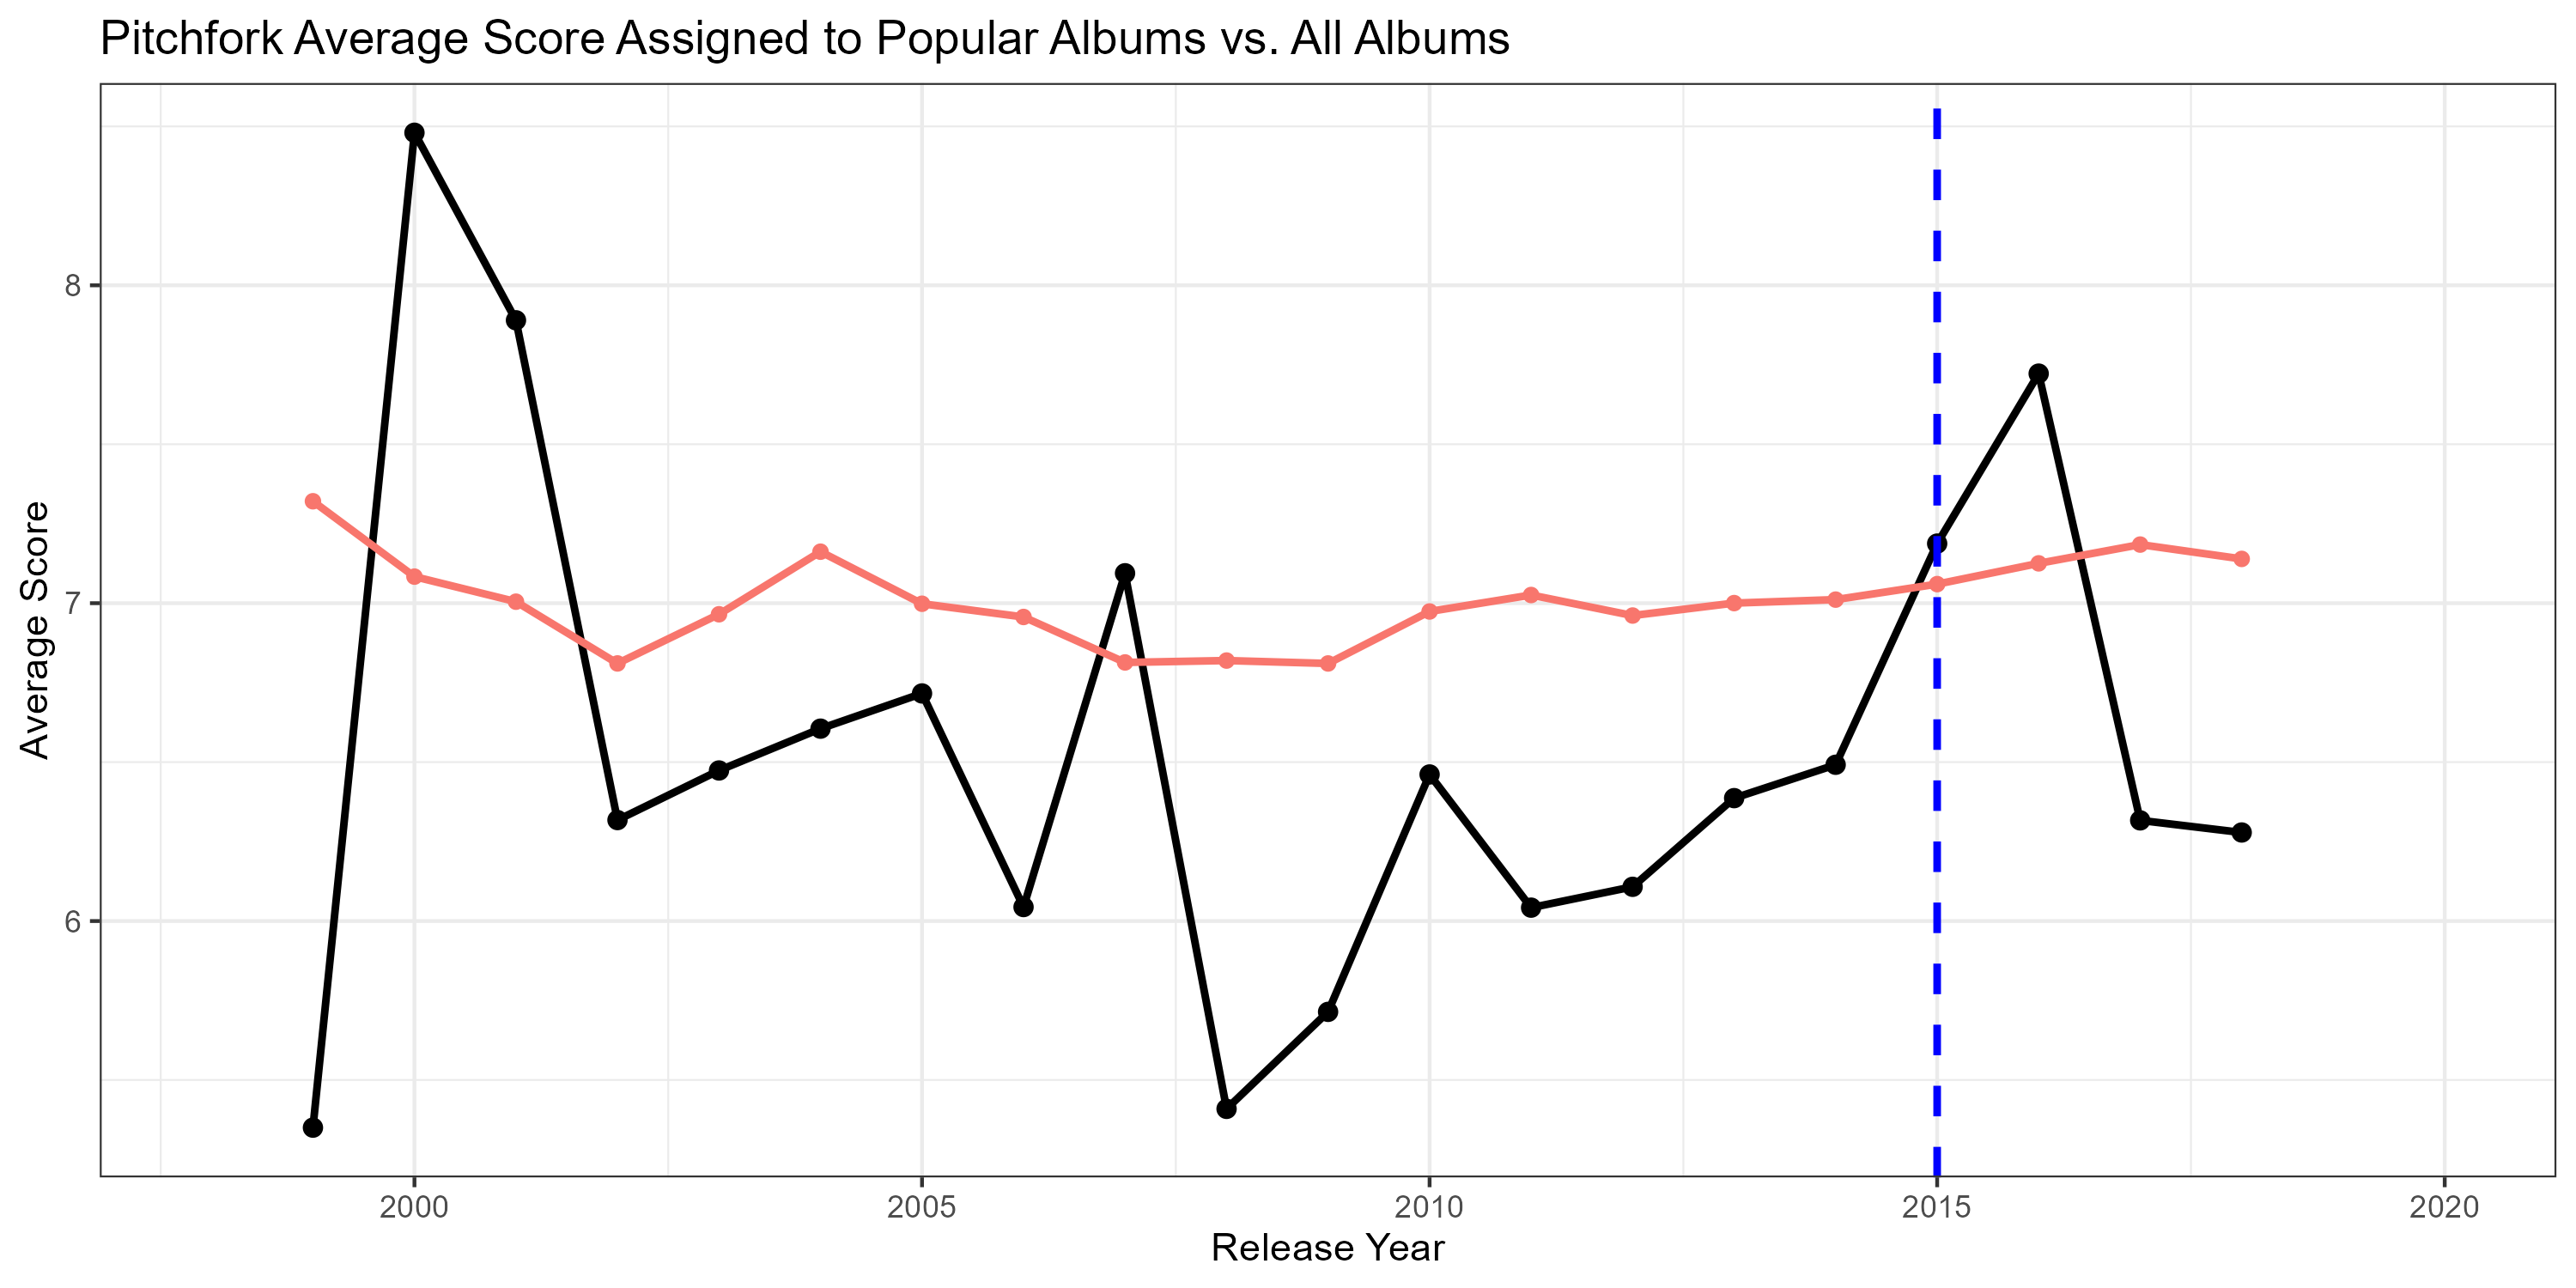
\includegraphics[width = \linewidth]{"figures/contrarian_index.png"}

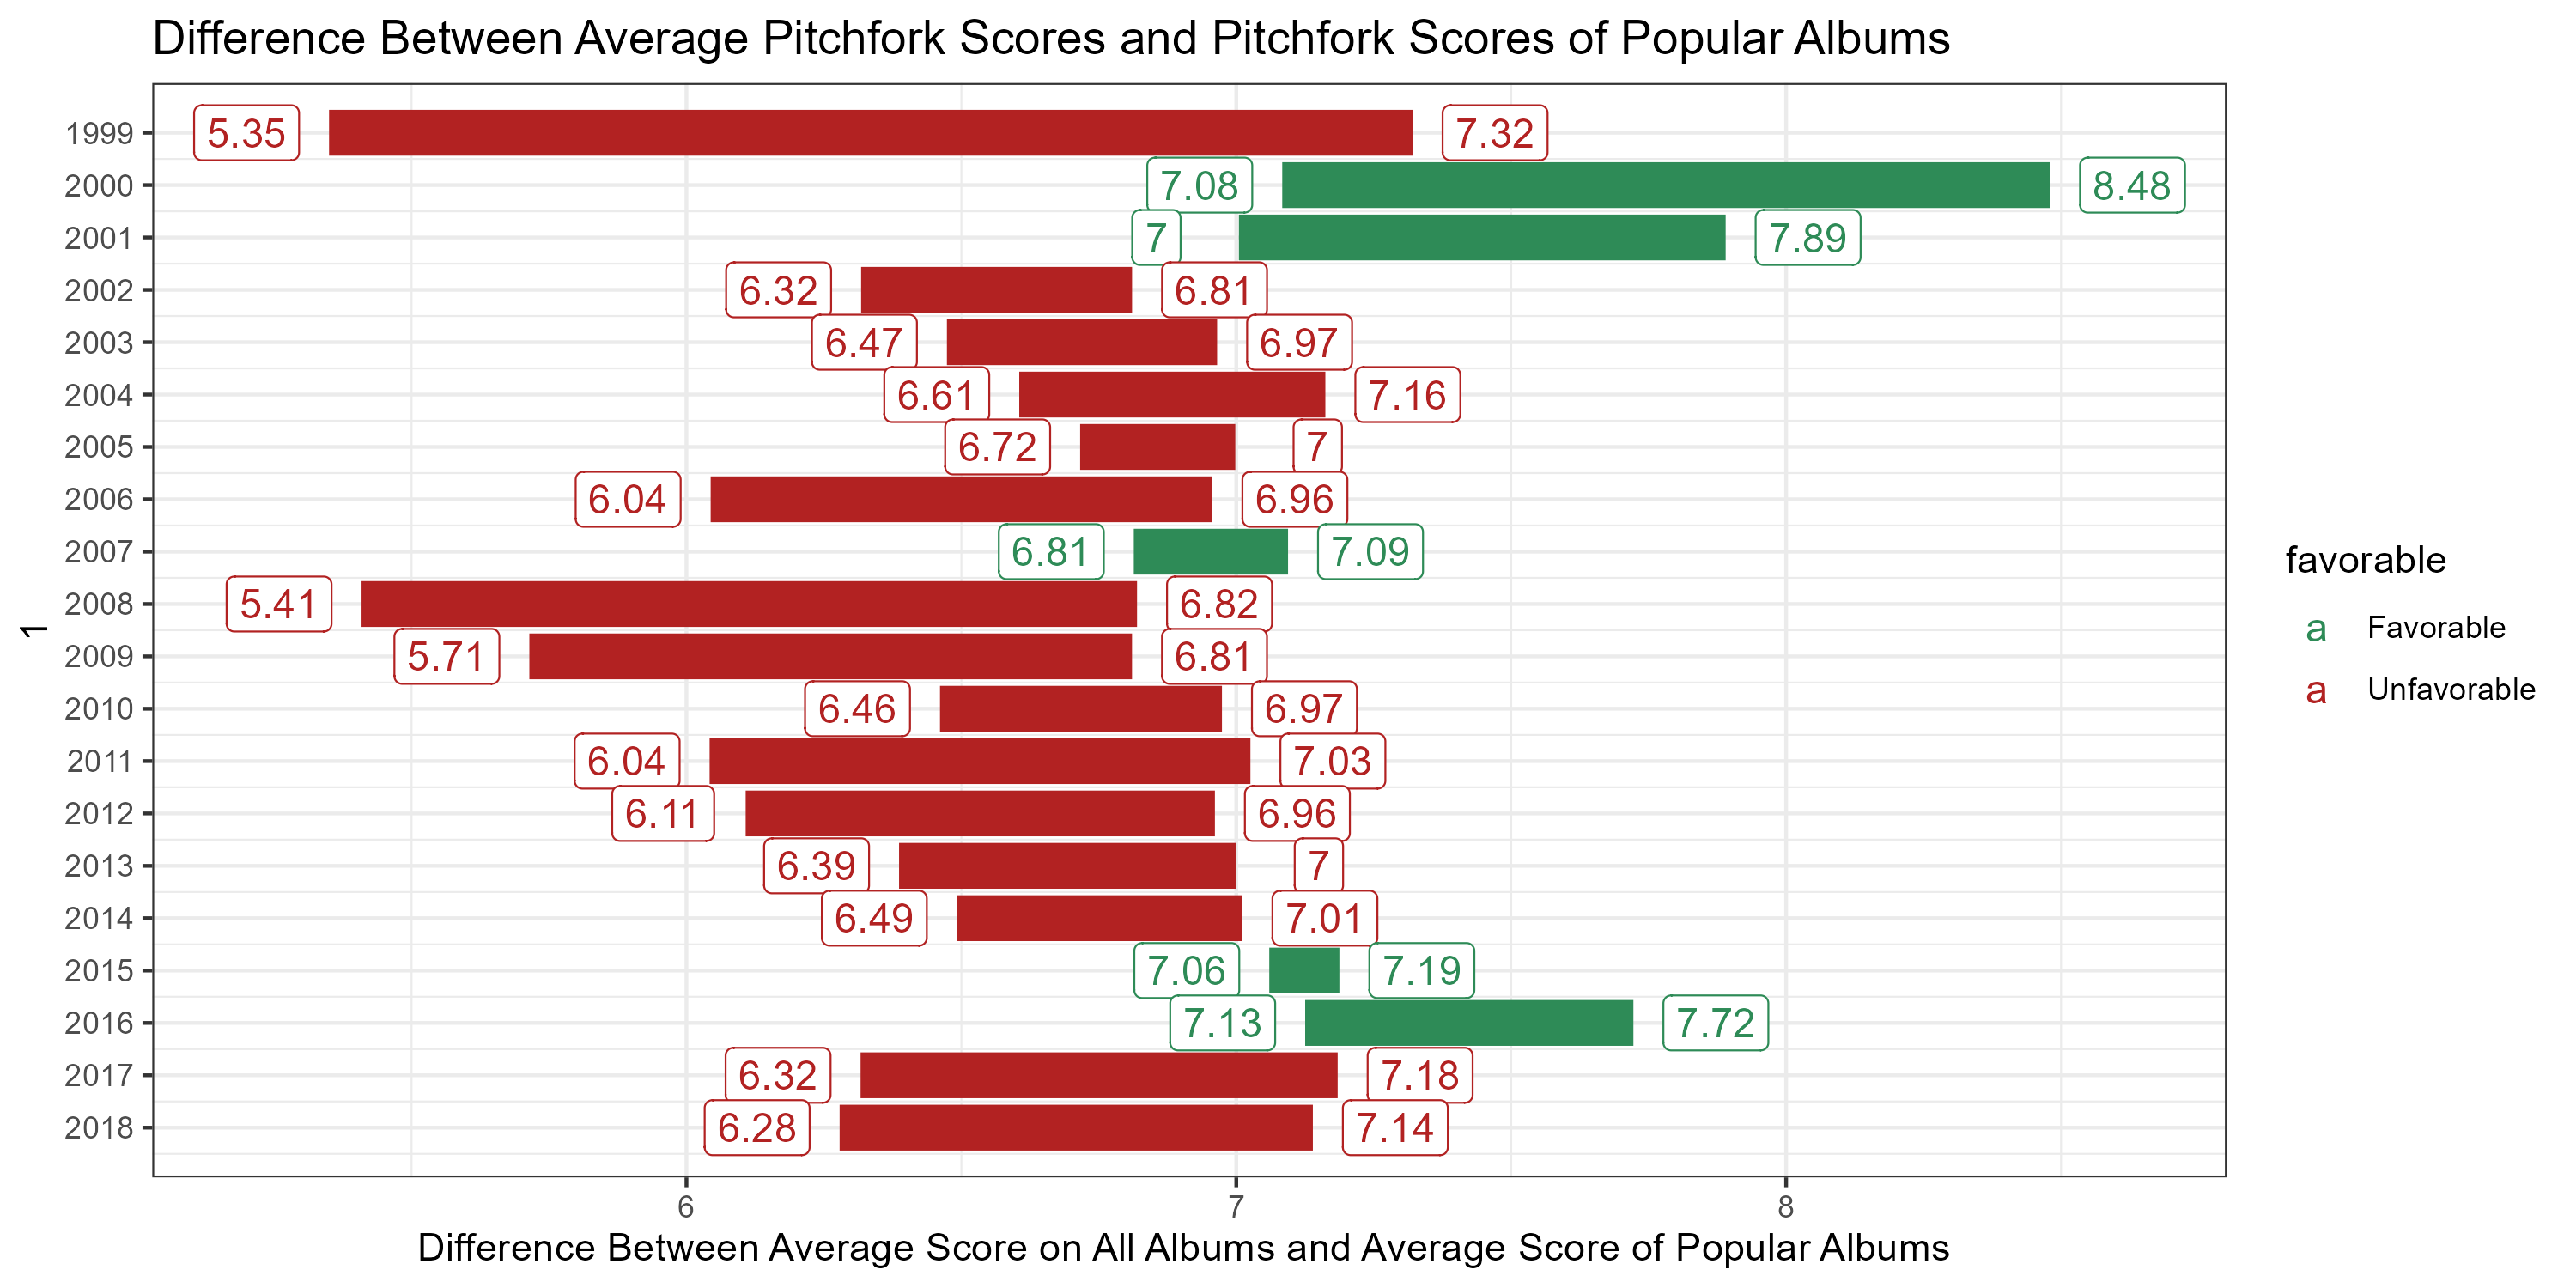
\includegraphics[width = \linewidth]{"figures/contrarian_index_bar.png"}

\subsection{Trends Post Conde-Nast Acquisition}
\subsubsection{Further Analysis}

\section{A Third Analysis: Perhaps Some Natural Language Processing}
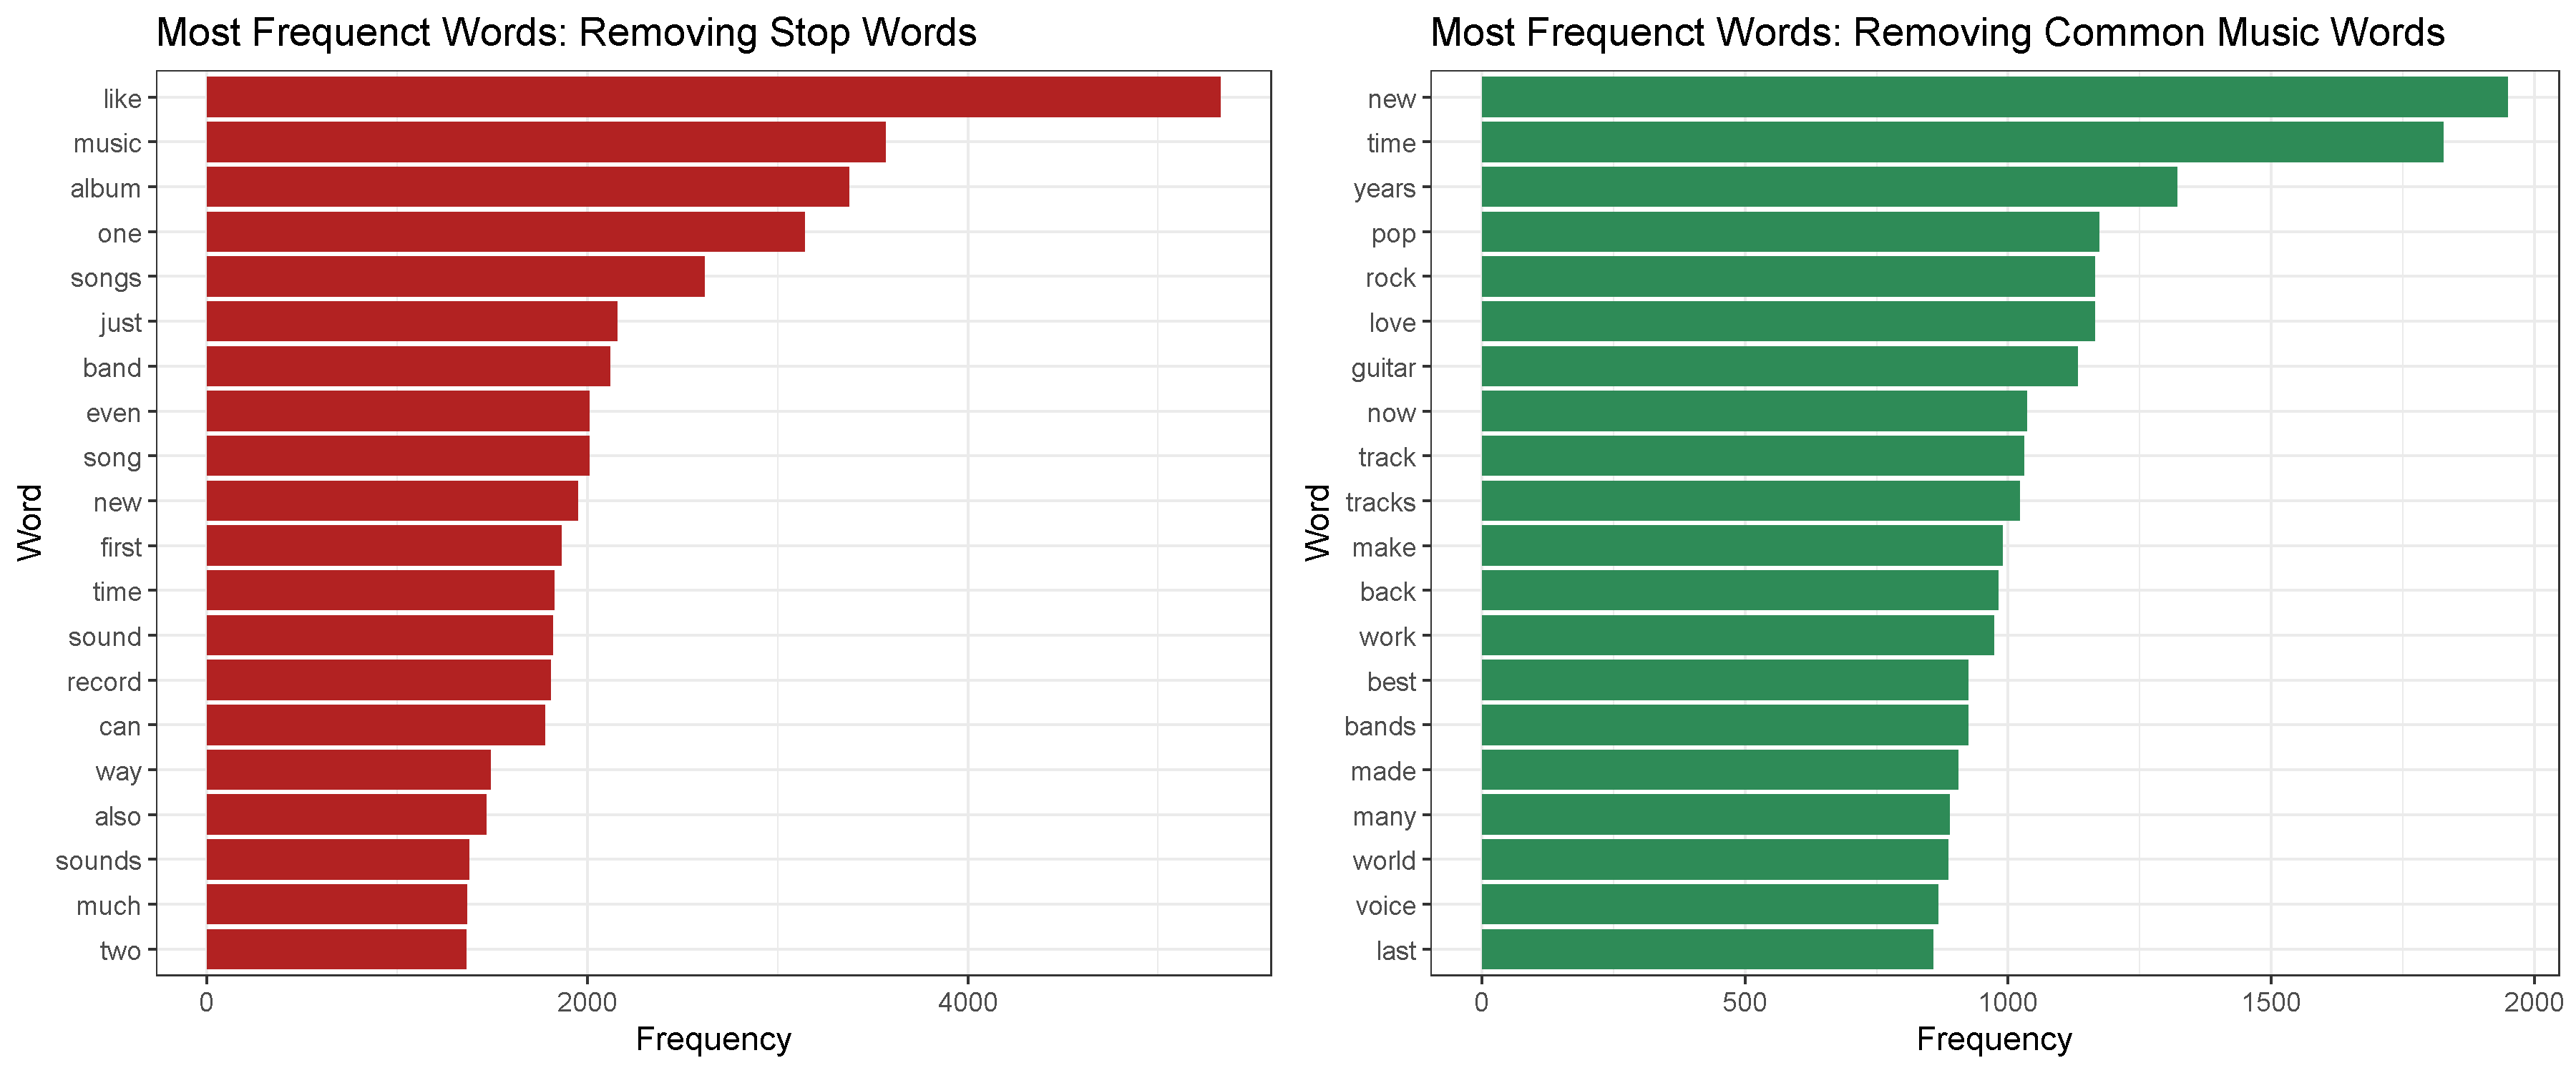
\includegraphics[width = \linewidth]{"figures/word_distribution_plot.png"}

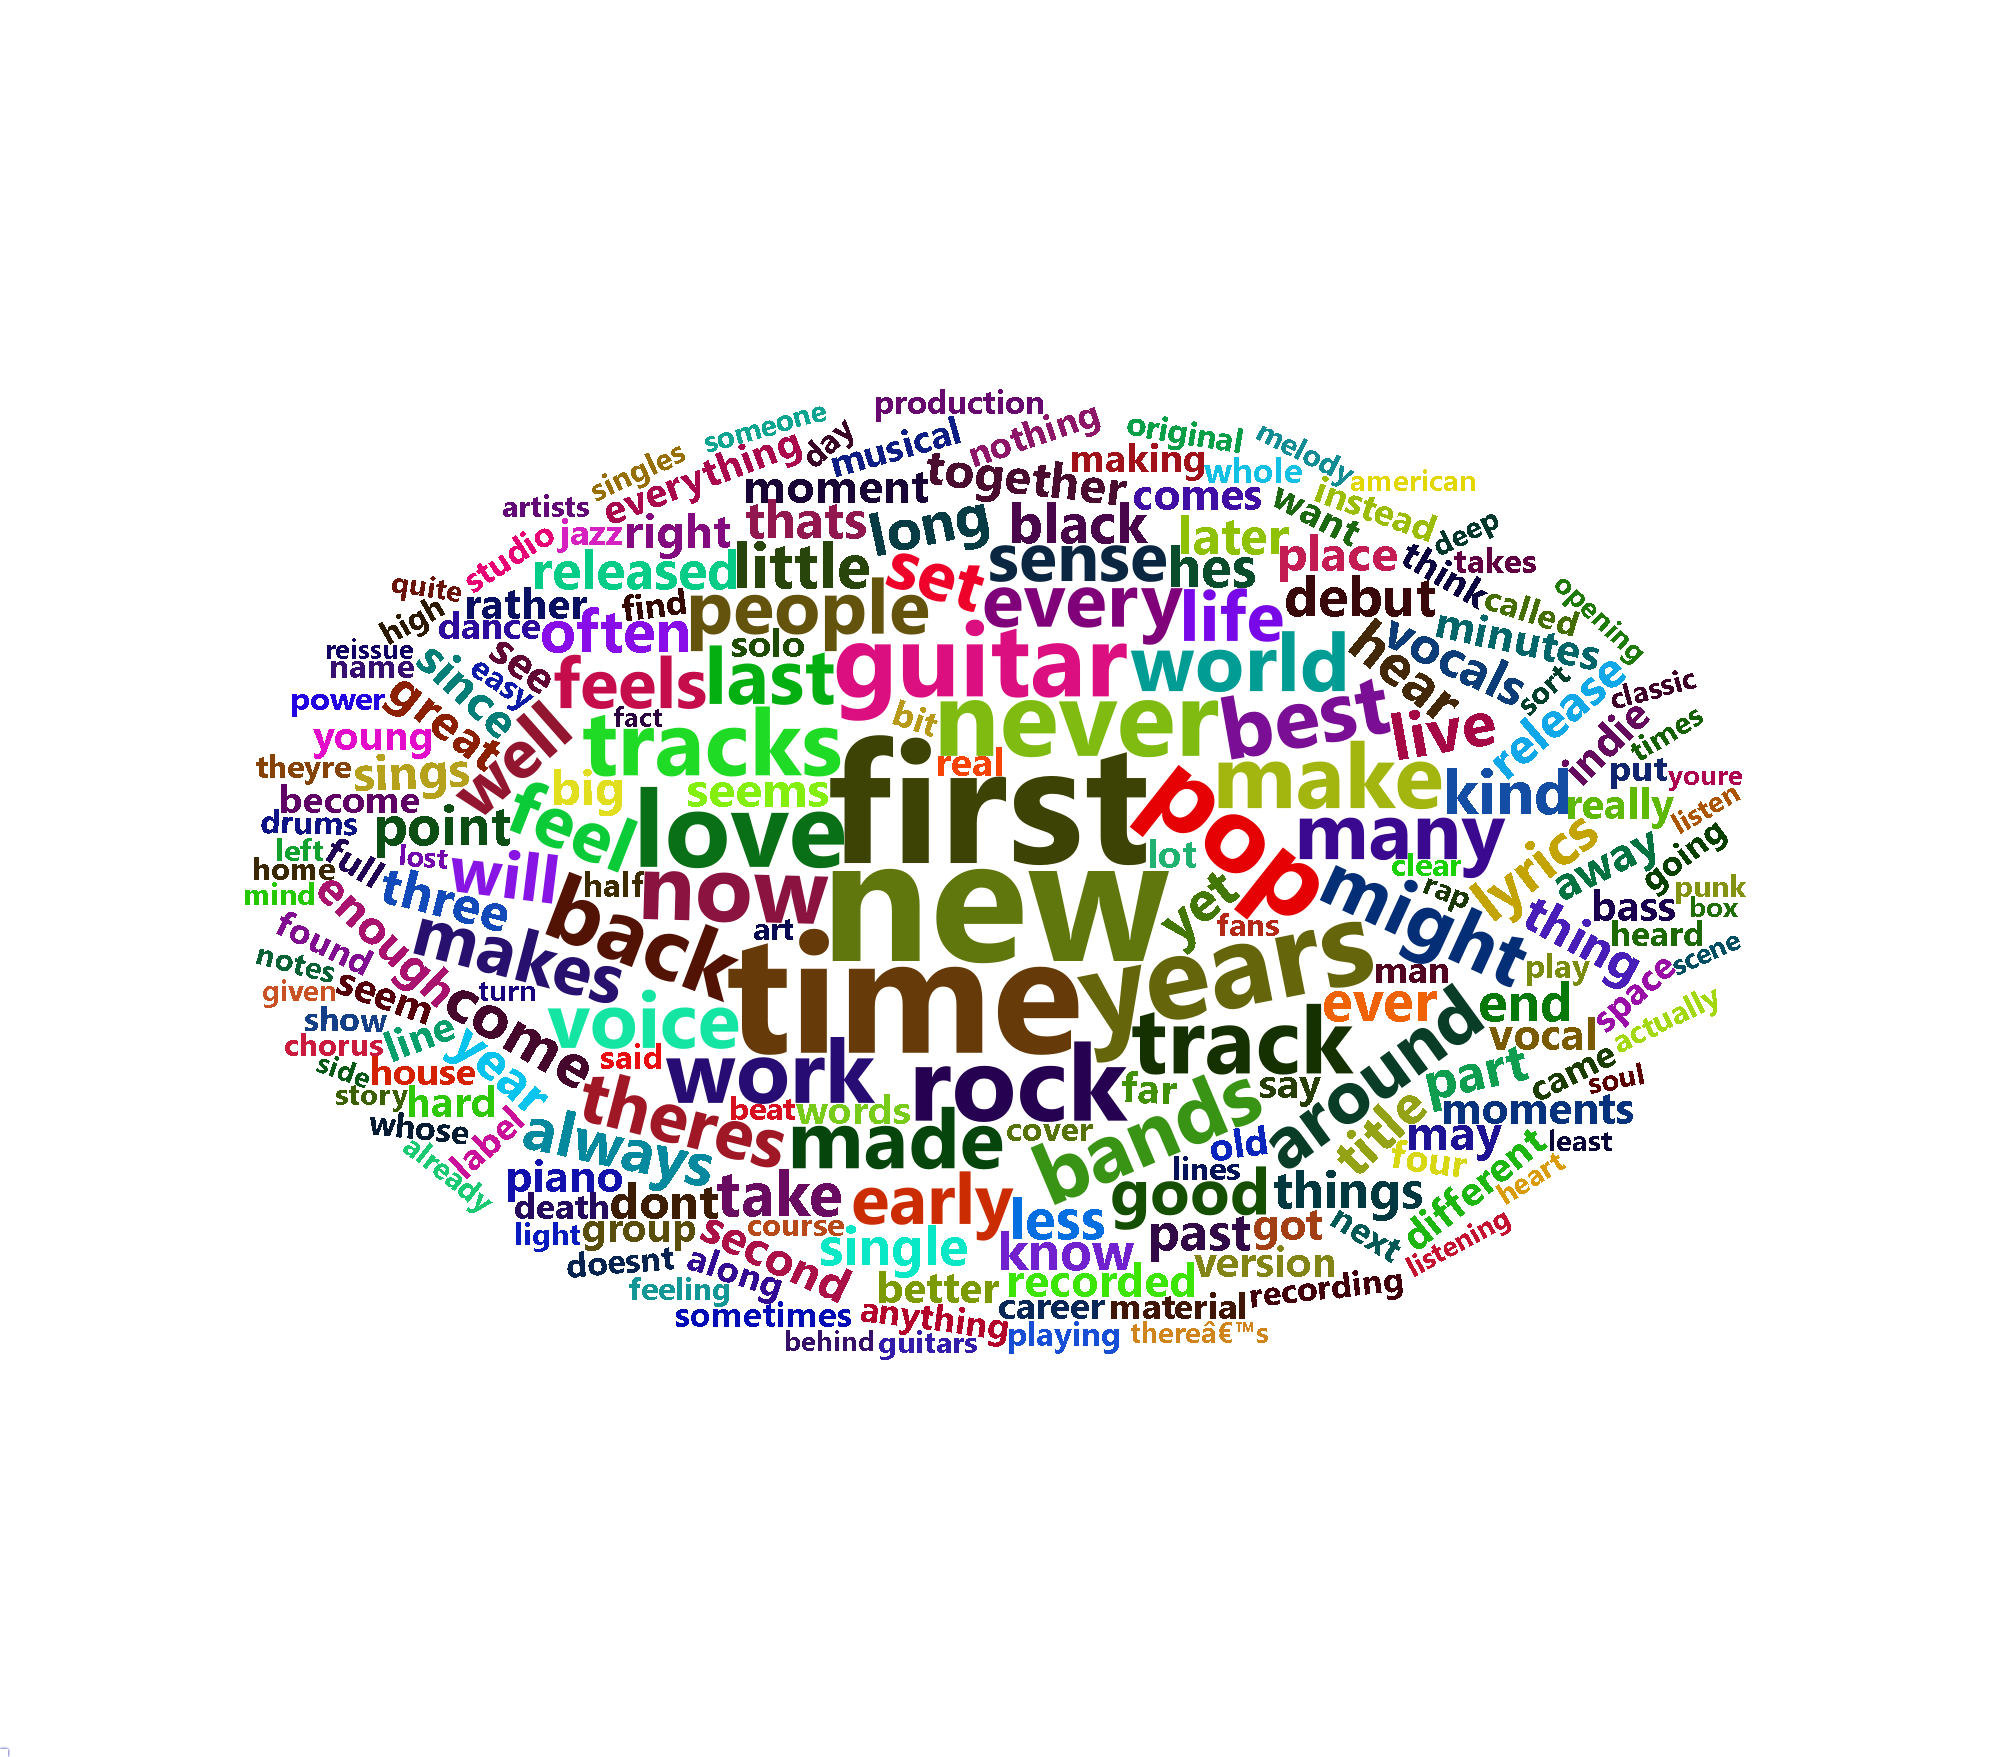
\includegraphics[width = \linewidth]{"figures/wordcloud.png"}

\subsection{Latent Dirichlet Allocation}

\section{Conclusion}
%
%\section{Section 1}
%\subsection{Subsection 1}
%\subsubsection{Subsubsection 1}
%You won't find subsubsubsections but you can also add a paragraph
%\paragraph{Paragraph} 
%
%if you really need another layer.
%
%But you can also modify the document if you really need more subsections.
%
%\section{Examples} \label{sec:section2}
%
%This is how you reference labels. Section \ref{sec:section2} explains how to reference labels. Section \ref{sec:citing} explains how to cite papers.
%
%\subsection{Citing}\label{sec:citing}
%This is one citation \cite{Mabuchi2012}. This is another citation \cite{HAN201687}. You can aggregate citations \cite{Mabuchi2012, HAN201687}.
%
%\subsection{Theorem}
%\begin{theorem} \label{theo:theorem1}
%	This is one way to define a theorem
%\end{theorem}
%
%You can also reference the Theorem \ref{theo:theorem1}.
%
%\subsection{Coloring text for revision}
%\textcolor{red}{You can color your text in case you want to add comments during the review of your comp I}.
%
%\subsection{Adding images}
%This is how you reference an image Figure \ref{fig:example_1}.
%
%\begin{figure}[ht]
%	\centering
%%	\includegraphics[width = 0.3\linewidth]{figures/Thesis_Defence.png}
%	\caption{You can cite the source in the caption \cite{barbour1}.}
%	\label{fig:example_1}
%\end{figure}
%
%This is how you reference a sub-image Figure \ref{fig:a}.
%
%\subsection{Adding equations}
%
%Equation \ref{eq:euler} is Euler's favorite equation. Maybe you want to cite as IEEE style? \eqref{eq:euler} shows Euler's favorite equation.
%
%\begin{equation}
%	\label{eq:euler}
%	e^{i\pi} + 1 = 0
%\end{equation}
%
%\subsection{Adding tables}
%
%Table \ref{tab:table1} is a simple table.
%\begin{table}[H]
%	\caption{This is a simple table}
%	\label{tab:table1}
%	\centering
%	\begin{tabular}{lccc}
%		\toprule
%		Class       &   Feature 1   &   Feature 2   &   Feature 3   \\
%		\midrule
%		Class 1     &   a   &   a   &   a   \\
%		Class 2     &   a   &   a   &   a   \\
%		\bottomrule
%	\end{tabular}
%\end{table}
%
%
%Table \ref{tab:table2} contains more advanced components.
%\begin{table}[H]
%	\caption{This is a comprehensive table}
%	\label{tab:table2}
%	\centering
%	\begin{tabular}{lcccc}
%		\toprule
%		& \multicolumn{2}{c}{CNN} & \multicolumn{2}{c}{CNN+LSTM} \\
%		\cmidrule(r){2-3} \cmidrule(r){4-5}
%		Difficulty     & Model 1 &  Model 2 & Model 1 & Model 2\\
%		\midrule
%		Easiest   & \Centerstack{ calm \\ angry \\ neutral}  &   \Centerstack{ angry \\ disgust \\ surprised}   &   \Centerstack{ calm \\ angry \\ neutral} & \Centerstack{ angry \\ fearful \\ calm} \\
%		\midrule
%		Hardest & \Centerstack{ sad \\ surprised \\ happy}   & \Centerstack{ neutral \\ sad \\ happy/fearful} & \Centerstack{ sad \\ surprised \\ happy/disgust}   &   \Centerstack{ neutral/sad \\ happy \\ disgust } \\
%		\bottomrule
%	\end{tabular}
%\end{table}
%
%
%\subsection{Lists}
%This is an unordered list
%\begin{itemize}
%	\item Item 1
%	\item Item 2
%\end{itemize}
%
%This is an ordered nested list
%\begin{enumerate}
%	\item Item 1
%	\begin{enumerate}
%		\item Item one
%		\item Item two
%		\item Item three
%	\end{enumerate}
%	\item Item 2
%\end{enumerate}
%
%\subsection{Algorithms}
%
%Algorithm \ref{alg:algorithm1} shows how to write pseudocode.
%
%\begin{algorithm}
%	\KwResult{Write here the result }
%	initialization\;
%	\While{While condition}{
%		instructions\;
%		\eIf{condition}{
%			instructions1\;
%			instructions2\;
%		}{
%			instructions3\;
%		}
%	}
%	\caption{Example of algorithm}
%	\label{alg:algorithm1}
%\end{algorithm}
%
%You can also import code, if you really need to show the exact code that you used. For example, Algorithm \ref{listing:research} shows how to do research.



%	\input{sections/conclusion}
	
	
	
	
	%If you came here because you want your references in a new page, uncomment the following line
	
	%\clearpage % If you want the references in a separate page
	\bibliography{bibliography}
	
	\clearpage % If you want the appendix in a separate page
	\appendix
%	\input{sections/appendix}

\begin{thebibliography}{}
\bibitem{ref1}
Rockwell, E. M., \& Rockwell, E. M. (2021). \emph{This is a citiation I made up} (Vol. 4). Prestigious Journal.


\end{thebibliography}
	
\end{document}
